La r\'ealisation de notre \'etude passe par la g\'en\'eration de $500$ graphes de flots $G$ de $30$ sommets ayant un degr\'e maximal moyen $\Delta(G) = 5$ qui simulent le fonctionnement d'un r\'eseau \'electrique. Nous en d\'eduisons \'egalement $500$ line-graphes de $150$ sommets et $470$ ar\^etes, en moyenne. \newline
Nous introduisons trois param\`etres $k, p\_correl, prob$:
\begin{enumerate}
\item $k$ d\'esigne le nombre de corr\'elations erron\'ees \`a ajouter dans la matrice $matE$. Dans notre \'etude, $k \in [1,9]$.
\item $p\_correl$ d\'esigne la probabilit\'e d'ajouter des erreurs de corr\'elations, soit corr\'elation {\em fausses positives} (ajout d'ar\^etes) soit corr\'elation {\em fausses n\'egatives} (suppression d'ar\^etes) soit les deux. Cette variable $p\_correl \in [0,1]$ varie par pas de $0.1$. Ainsi,
	\begin{itemize}
	\item si $p\_correl=0$ $\rightarrow$ la matrice $matE'$ ne contient que des  corr\'elations {\em fausses positives} car on supprime uniquement des ar\^etes dans le line-graphe de matrice d'adjacence $matE$.
	\item si $p\_correl=0.5$ $\rightarrow$ le nombre de corr\'elations {\em fausses n\'egatives} et  {\em fausses positives} est approximativement identique  dans la matrice $matE'$ car on ajoute et supprime \'equiprobablement des ar\^etes dans la matrice $matE$.
	\item si $p\_correl=1.0$ $\rightarrow$ la matrice $matE'$ ne contient que des corr\'elations {\em fausses n\'egatives} car on ajoute des ar\^etes dans le line-graphe de matrice $matE$.
	\end{itemize}
\item $prob$ d\'esigne la probabilit\'e associ\'ee \`a une corr\'elation selon le type d'erreurs rencontr\'e dans $matE'$. En un mot, $prob$ est la valeur de corr\'elation entre ar\^etes.
Ce param\`etre est important car les valeurs de corr\'elations calcul\'ees  ne sont pas binaires mais dependent d'une loi de probabilit\'e. Nous en reparlerons \'egalement dans la section \ref{fonctionDeCout}.
\end{enumerate}
Pour ajouter des erreurs de corr\'elation \`a la matrice $matE$ correcte, on tire al\'eatoirement $k$ cases non encore modifi\'ees. Nous mettons chaque case et sa case sym\'etrique \`a $1$ si la probabilit\'e de la case est inf\'erieure ou \'egale \`a $p\_correl$. Si cette case est d\'ej\`a \`a $1$, on choisit une autre case. Selon le type d'erreurs de chaque case (vrai n\'egatives, vrai positives), on lui attribue une valeur de corr\'elation selon les distributions pr\'ed\'efinies.
\newline

Consid\'erons le graphe $G_k$ de matrice d'adjacence $matE_k$ dans laquelle on ajoute $k \in [1,9]$ erreurs de corr\'elation selon $p\_correl=0.5$, la probabilit\'e d'ajouter autant d'erreurs {\em fausses n\'egatives } que d'erreurs {\em fausses positives}. 
\`A la fin de l'ex\'ecution de l'algorithme de couverture, s'il existe des sommets de $G_k$ non couverts par {\em une ou deux cliques}, on les ajoute \`a l'ensemble des sommets \`a corriger $sommets\_1$ et nous appliquons l'algorithme  de correction sur chaque sommet de $sommets\_1$ selon les m\'ethodes suivantes:
\begin{itemize}
\item m\'ethode 1 : degr\'e minimum avec remise.\newline
Elle consiste \`a s\'electionner le sommet de degr\'e minimum dans l'ensemble $sommets\_1$, \`a appliquer l'algorithme de correction afin de modifier $matE_k$ et enfin  d'ex\'ecuter \`a nouveau les deux algorithmes sur la matrice $matE_k$ modifi\'ee.
\item m\'ethode 2 : co\^ut minimum avec remise. \newline
Elle consiste \`a s\'electionner le sommet de co\^ut minimum dans l'ensemble $sommets\_1$, \`a appliquer l'algorithme de correction pour modifier $matE_k$ et enfin \`a re-ex\'ecuter les deux algorithmes sur la matrice $matE_k$ modifi\'ee.
\item m\'ethode 3 : co\^ut minimum avec permutation des sommets de $sommets\_1$. \newline
Elle consiste \`a choisir une permutation dont les sommets sont class\'es par ordre croissant de leur co\^ut  de modification de la matrice $matE_k$ et \`a appliquer l'algorithme de correction sur cette permutation.
\item m\'ethode 4 :  degr\'e minimum avec  permutation des sommets de $sommets\_1$. \newline
Elle consiste \`a choisir une permutation dont les sommets sont class\'es par ordre croissant de leur degr\'e et \`a appliquer l'algorithme de correction sur cette permutation.
\item m\'ethode 5 : permutation al\'eatoire des sommets de $sommets\_1$. \newline
Elle consiste \`a choisir al\'eatoirement $N$ permutations puis \`a appliquer l'algorithme de correction et \`a s\'electionner la permutation ayant un co\^ut et une distance de Hamming minimum.
\end{itemize}

% calcul de moy_dl et moy_dh
Consid\'erons 
  $\alpha \in [1, 5]$ le nombre de fois qu'on applique $k$ erreurs dans la matrice $matE$ du line-graphe $LG$,  
 $G_{k, \alpha}$ le graphe de matrice d'adjacence $matE_{k, \alpha}$ dont on a modifi\'e $k$ corr\'elations $\alpha$ fois et 
 $LG_{k, \alpha}$  le line-graphe de matrice d'adjacence $matE_{k, \alpha}$ fourni par les algorithmes de couverture et de correction \`a partir du graphe $G_{k, \alpha}$.
\newline
En comparant
\begin{enumerate}
\item  $LG$ et $LG_{k, \alpha}$, on obtient la distance de Hamming not\'ee $DH_{k,\alpha}$.
\item $G_{k,\alpha}$ et $LG_{k,\alpha}$, on obtient la distance line not\'ee $DL_{k,\alpha}$.
\end{enumerate}
On d\'efinit par les variables $moy\_DH$ et $moy\_DL$, les moyennes respectives des distances de Hamming (not\'ee $DH_{k,\alpha}$) et des distances line (not\'ee $DL_{k,\alpha}$) pour une valeur donn\'ee de $k$ et pour tout $\alpha \in [1, 5]$.
\begin{equation}
moy\_DH_k = \sum_{\alpha = 1}^{5} DH_{k, \alpha} \hspace{2 em}
moy\_DL_k = \sum_{\alpha = 1}^{5} DL_{k, \alpha}
\end{equation}

Le protocole d'exp\'erimentation est r\'esum\'e dans la figure \ref{recap_protocole_etude}. Le r\'eseau de flots $G$ g\'en\'er\'e est transform\'e en un line-graphe $LG$, puis $k$ erreurs de corr\'elations  sont ajout\'ees $\alpha$ fois dans $LG$ pour obtenir $G_{k,\alpha}$. Nous appliquons les algorithmes (couverture et correction) pour d\'eterminer la line-couverture (ou la plus proche possible) du graphe $G_{k,\alpha}$ car ce graphe n'est pas n\'ecessairement un line-graphe. Cette line-couverture forme un line-graphe $LG_{k, \alpha}$ proche ou identique au line-graphe $LG$. Le line-graphe $LG_{k, \alpha}$ est utilis\'e pour calculer les distances line ($DL_{k, \alpha}$) et de Hamming ($DH_{k, \alpha}$).
Les valeurs moyennes ($moy\_DL$, $moy\_DH$) des distances line et de Hamming sont calcul\'ees pour chaque erreur $k$ et leurs distributions sont pr\'esent\'ees dans la section suivante afin de montrer les performances des algorithmes en pr\'esence d'erreurs de corr\'elations de diff\'erentes lois de probabilit\'es.
\begin{figure}[htb!] 
\centering
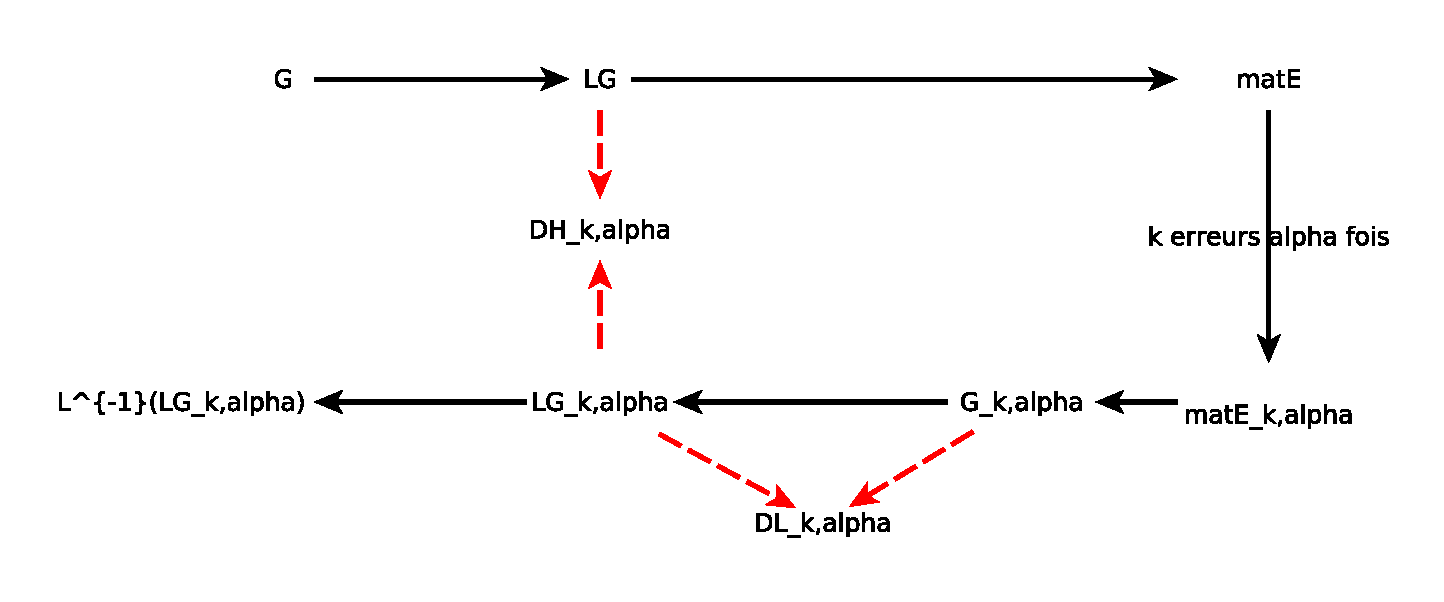
\includegraphics[scale=0.70]{recapProtocoleEtude.eps}
\caption{ Diff\'erentes \'etapes du processus d'exp\'erimentation de nos algorithmes (fl\`eches en noir), calcul de distances entre \'etapes (fl\`eches pointill\'ees en rouge).}
\label{recap_protocole_etude} 
\end{figure}
%---- decription protocole d'etude --> fin